\label{chap:sprint4}
In this chapter the planning and work-flow regarding Sprint 4 will be described. 
Everything from setting our goals to implementation and testing. At the end the team will evaluate the whole sprint and try on answer the following questions: What went well? What could be improved? 
\section{Sprint planning}

The team with the customer planned how to take the project further on a regular planning meeting.
At this point it was possible to send control signals to multiple clients, and then detect the screens that lit up. 
It was decided that the plan for this sprint was to combine those two modules, and try to display a short animation.
This meant that detection of possible clients' locations must be performed and than connecting its position in a grid with an appropriate socket linked with client.

After this locating, commands to all clients must be continuously send with information, what colors should they lit.
To be more efficient and do not use too much traffic, which could result into delays on network, it was proposed by customer that video should be preprocessed and large chunks of data with timing should be send to clients.

Next, the team with the customer discussed long term planning of the product.
Since this product cannot be finished and deploy for everyday and commercial use due to time restriction, the features included and not included in final prototype were discussed.
The customer proposed two different goals.
One involved mobile device tracking (on rock concert after detection phase, it is probable, that audience wont be static but they will be moving, and therefore if animation should be displayed in proper way, these movements should be detected).
After a short discussion, it was decided that this is a long term goal, which is out of scope of this project.
The focus was put on finishing all core modules and therefore a different goal was adopted.
This goal will be described in Section \ref{sec:sprint4goal}.

As the team wanted the customer feedback more often, it was again settled, than a next pre-delivery demonstration will be made for meeting on 17th of October. 

All implementation related stories for sprint 4 are presented in Table \ref{tab:sprint4stories}.
%\caption{User stories selected for Sprint 4.}
  \label{tab:sprint4stories}
 \def\arraystretch{1.25}
 
\begin{longtable}{ccXcc}

\toprule[0.5mm]
\multirow{2}{*}{\textbf{ID}} &
\multirow{2}{*}{\textbf{Ref.}} & \multirow{2}{*}{\textbf{Description}} & \multicolumn{2}{c}{\textbf{Hours}} \\
 					& & & \textbf{Est.} & \textbf{Sp.} \\
%\textbf{ID} 	& \textbf{Description} 	& \textbf{Est.} & \textbf{Sp.} \\
\midrule
\textbf{I4.1} 	& 	& {\bf As a server I need to link the devices' location with their ids.}	 &  52	& \textbf{48} \\

\textbf{I4.2} 	& 	& {\bf As a server I need to identifiy multiple clients from light.}		 &  19	& \textbf{18} \\

\textbf{I4.3} 	& 	& {\bf As a server I need to map all available devices to grid.} 			 & 22 & \textbf{18} \\	

\textbf{I4.4} 	& 	& {\bf As a server I need to play the whole media to the grid.} 			 & 37 & \textbf{34} \\
	
\midrule
		
				&& \textbf{SUM:}		&		130	& \textbf{136}
 \\																			
\bottomrule[0.5mm]
\end{longtable}



In sprint 4 the team also planned to work more on the report. 
The plan was to finish sprint 3, since that sprint itself finished the week before. 
It was also wanted to start working on sprint 4 in report.
Since more modules were implemented and their integration must be done, discussion about architecture started to be intensive.
The main goal was to keep architecture as general as possible and open for all future (out of scope) features.
Therefore the idea of architecture become more clear and work on writing architecture chapter could start.
The team where also getting a better understanding of what the end product would look like, therefore it was planned to start working a little bit on the evaluation as well. 
The supervisor also came up with some suggestions for small improvements on the report, which the team planned to follow up.
Also it was decided to make to the user stories more consistent. 
Last but not least, it was also planned to separate the implementation stories from the documentation, and the project management stories.

All the documentation related stories for sprint 4 are presented in Table \ref{tab:sprint4Documentationstories}.
%\caption{User stories selected for Sprint 2.}
\def\arraystretch{1.25}
 
\begin{longtable}{ccXcc}
\label{tab:sprint2Documentationstories}\\[-6mm]
\caption{Documentation stories selected for sprint 2}\\[-4mm]
\toprule[0.5mm]
\multirow{2}{*}{\textbf{ID}} &
\multirow{2}{*}{\textbf{Ref.}} & \multirow{2}{*}{\textbf{Description}} & \multicolumn{2}{c}{\textbf{Hours}} \\
 					& & & \textbf{Est.} & \textbf{Sp.} \\
%\textbf{ID} 	& \textbf{Description} 	& \textbf{Est.} & \textbf{Sp.} \\
\midrule


\textbf{D2.1} 	& 
	\refwbs{wbs_documentation}{WBS 8.2}	& {\bf As a student I need to finish the pre-study chapter.} 									& 	12	& \textbf{ 16} \\

\textbf{D2.2} 	& 
	\refwbs{wbs_documentation}{WBS 8.2}	& {\bf As a student I need to finish the planning chapter.} 									& 	10	& \textbf{ 14} \\

\textbf{D2.3} 	&
	\refwbs{wbs_documentation}{WBS 8.2} 	& {\bf As a student I need to finish requirements chapter.} 									& 	30	& \textbf{ 26} \\

\textbf{D2.4} 	& 
	\refwbs{wbs_documentation}{WBS 8.2}  & {\bf As a student I need to finish the architecture chapter.} 								& 	24	& \textbf{ 12} \\

\textbf{D2.5} 	& 
	\refwbs{wbs_documentation}{WBS 8.2}	& {\bf As a student I need to finish sprint 1 chapter.} 										& 	12	& \textbf{ 16} \\

\textbf{D2.6} 	& 
	\refwbs{wbs_documentation}{WBS 8.2}	& {\bf As a student I need to work on the  sprint 2 chapter.} 									& 	16	& \textbf{ 18} \\
%ASK group about this:
%\textbf{360} 	& \refreq{}
%	& {\bf As a student I need to start on the architechture chapter.} 								& 	?	& \textbf{ ?} \\	

								
\hline
				&& \textbf{SUM:}		&		104	& \textbf{102}
 \\																			
\bottomrule[0.5mm]
\end{longtable}


All the project management related stories for sprint 4 are presented in Table \ref{tab:sprint4storiesProcess}.
%\caption{User stories selected for Sprint 1.}
\label{tab:sprint1storiesProcess}
\def\arraystretch{1.25}
 
\begin{longtable}{ccXcc}

\toprule[0.5mm]
\multirow{2}{*}{\textbf{ID}} &
\multirow{2}{*}{\textbf{Ref.}} & \multirow{2}{*}{\textbf{Description}} & \multicolumn{2}{c}{\textbf{Hours}} \\
 					& & & \textbf{Est.} & \textbf{Sp.} \\
%\textbf{ID} 	& \textbf{Description} 									& \textbf{Est.} & \textbf{Sp.} \\
\midrule

% === Process ==========================
\textbf{326} 	& 
	& {\bf  As a student I have to track effort time} 	& 		16	& \textbf{16} \\
\textbf{345} 	& 
	& {\bf As a student I have attend the weekly meetings with the customer} 	
	& 	22	
	& \textbf{?} \\
		&& Preparation for demonstration	& 2 & ? \\
		&& Demonstration	& 6 & ? \\
		&& Writing minutes 	&  6 & ? \\	
		&& Customer meeting	&  6 & ? \\
		&& Writting minutes	&  2 & ? \\
		
\textbf{327} 	& 
	& {\bf As a student I have to attend the weekly meetings with the supervisor} 	
	& 	12	
	& \textbf{?} \\
		&& Meeting in week I	& 4 & ? \\
		&& Meeting in week II	& 4 & ? \\
		&& Writing minutes from week I 	&  2 & ? \\
		&& Writing minutes from week II	&  2 & ? \\	

\textbf{344} 	&& {\bf As a student I need to attend the team building.} 	& 		7	& \textbf{9} \\
		

\textbf{321} 	&& {\bf As a student I need to participate to lectures about team dynamics. } 	& 		32	& \textbf{25} \\
				&& Course of group dynamics Thu.	&  &  \\
				&& Summary of course and exchange learned.	&  &  \\				
				
\hline
				&& \textbf{SUM:}		&		164	& \textbf{?}
 \\																			
\bottomrule[0.5mm]
\end{longtable}


% hous all in total: Estimated: 130 + 65 + 42 = 237  Spent: 136+ 36+35= 207

\subsection{Duration}
This sprint is 2 weeks long. From 14th of October 2013 to 27th of October 2013. 
We agreed on the date of presentation and showing the running demo -- on Thursday 25th of October 2013.
Estimated velocity is 200 hours since we agreed on 25 working hours per person per week.

\section{Sprint goal}
\label{sec:sprint4goal}
The goal of this sprint is to have application which integrates already implemented modules.
This application should be able to display using clients a short animation of a traffic light as can be seen in Figure \ref{fig:trafficlight}.
This is in fact prototype 4 -- \emph{Traffic light control} as can be seen in Section \ref{sec:milestones}.

\begin{figure}[h]
	\centering
		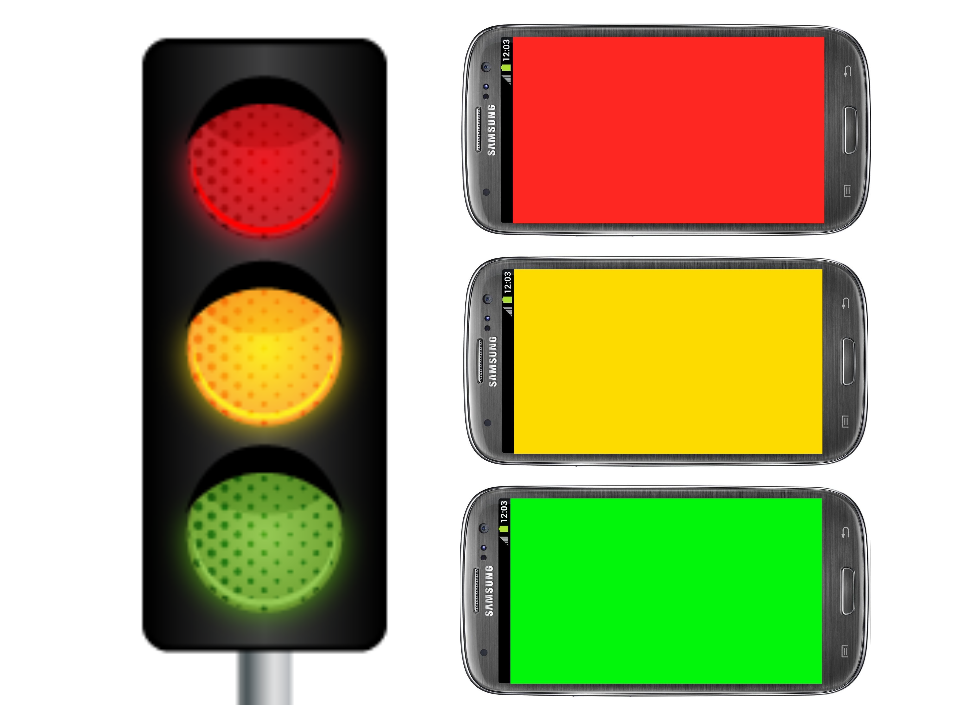
\includegraphics[width=10cm]{sprint4/trafficlight.png}
	\caption{Traffic light}
	\label{fig:trafficlight}
\end{figure}

\section{Architecture}
In this section it will be described architecture for sprint 4 using 4+1 view model.
The implementation work can be divided into two logical parts: linking clients' sockets with their position in grid and processing media (animation) into chain of commands for clients.
Therefore the architecture description will be in each view divided into two parts.

\subsection{Logical view}
In Figure \ref{fig:class_diagram_device_sprint4} can be seen class diagram of device locating component.
On the top of the hierarchy there is an interface \texttt{DeviceLocatingStrategy}, which defines common behavior for two classes: \texttt{DeviceMapper} and \texttt{DeviceTracker}.
The first mentioned is an abstract class and defines shared behavior for all (future) types of implementations of linking sockets with positions.
One of these classes is \texttt{DeviceMapperSimple} which uses simple dummy algorithm.
This algorithm simply let lit clients with white color one by one and detects this color.
Detected tile is position of a mobile device.

Class \texttt{DeviceTracker} is class that is used as a getter of list of devices with their positions.
Core of this class is missing, it is only present so it can be extend as a future feature.
Future purpose of this class is to track already detected devices and update their positions during playing media.

\begin{figure}[h]
	\centering
		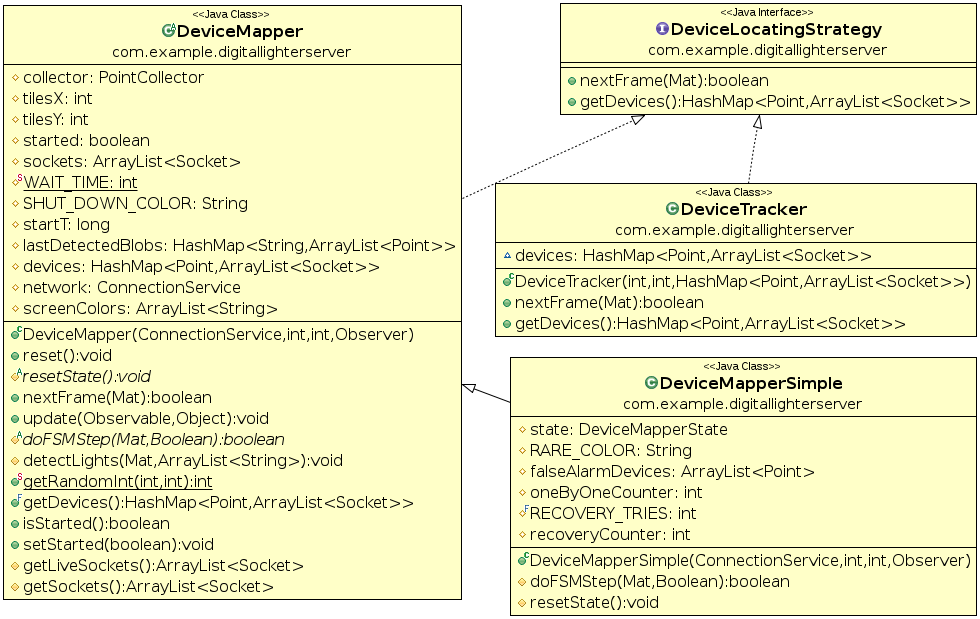
\includegraphics[width=16.2cm]{sprint4/class_diagram_device.png}
	\caption{Sprint 4 device locating module}
	\label{fig:class_diagram_device_sprint4}
\end{figure}

In Figure \ref{fig:class_diagram_device_sprint4b} you can see class diagram of second component -- media player.
Class \texttt{ImageMapper} is responsible for loading single pictures.
These pictures are used by class \texttt{CommandCreator}, which can create commands generically during run
and as a parameter can be passed number of frames that should be parsed in advance and send to client in single command.
For sending to clients in appropriate moments is responsible instance of class \texttt{MediaPlayer}.
As you can see, the \texttt{MediaPlayer} class keeps an instance of class \texttt{DeviceLocatingStrategy} which servers as a getter for sockets and positions.
\begin{figure}[h]
	\centering
		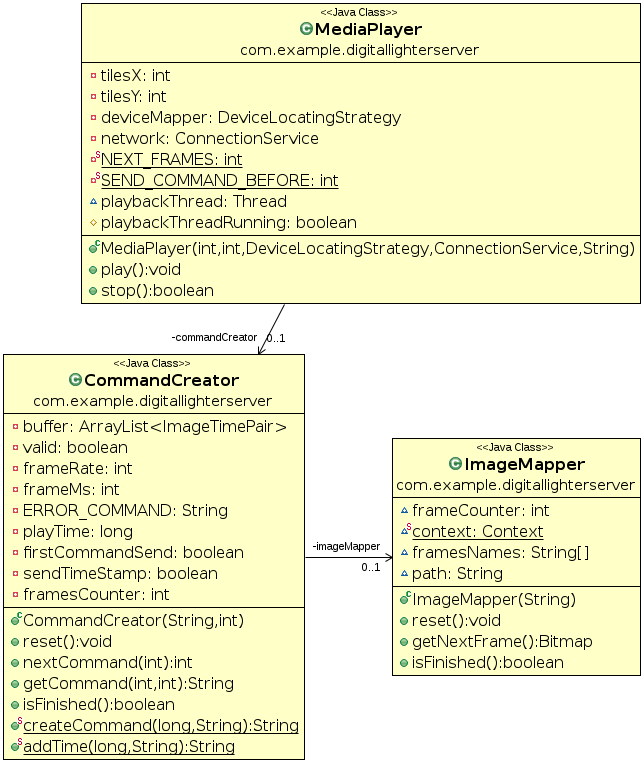
\includegraphics[width=11.0cm]{sprint4/class_diagram_media_player.png}
	\caption{Sprint 4 media player module}
	\label{fig:class_diagram_device_sprint4b}
\end{figure}


\subsection{Physical view}
In this sprint, no changes were made in physical view.
Therefore you can see the physical view in deployment diagram in Figure \ref{fig:sprint3_deployment_diagram} from sprint 3.

\subsection{Process view} \label{txt:sprint4_processview}
Process view for sprint 4 can be seen in activity diagram in Figure \ref{fig:sprint4_activity_diagram}.
First, to all clients is sent control signal to lit with black color.
After some delay (because of possible network delay, there is need for waiting), all white blobs are detected, this represents \emph{false alarm} blobs.
Next, iterating through all clients starts.
In each iteration to only one clients is sent to lit with white color.
Again, after some delay a new detection is performed and difference between currently detected white blobs and false alarm blobs is calculated.
The difference is a position of client.

It should be mentioned, that both activities \emph{Detect white color} are in fact slightly modified subactivities, which can be seen in Figure \ref{fig:sprint3_activity_diagram}.
Therefore this diagram in Figure \ref{fig:sprint4_activity_diagram} is subactivity of activity \emph{Detect clients location} of Figure \ref{fig:activity_diagram_server}.
\begin{figure}[h]
	\centering
		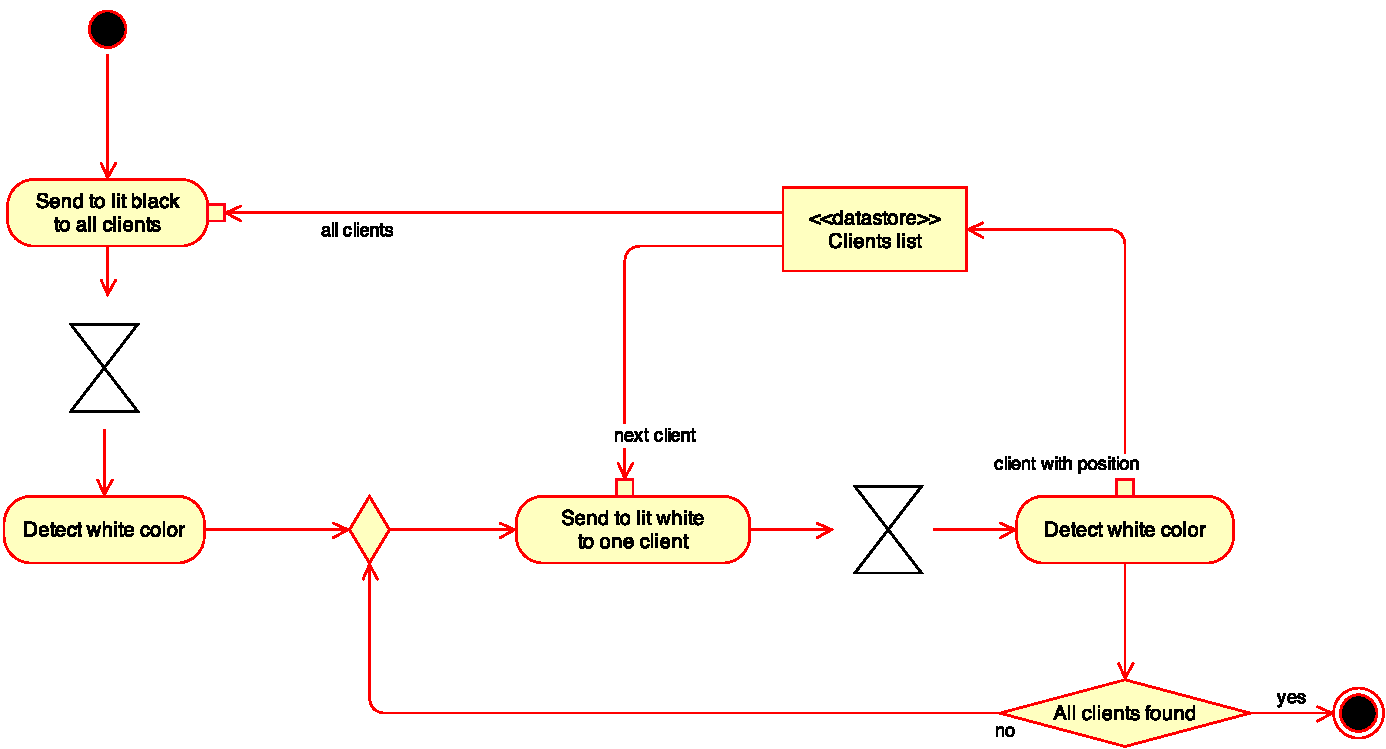
\includegraphics[width=16.2cm]{sprint4/activity_sprint4.pdf}
	\caption{Sprint 4 activity diagram}
	\label{fig:sprint4_activity_diagram}
\end{figure}

The media player component is from point of process view rather straightforward, and therefore there will be no figure presented.

\section{Testing}
There was no unit testing for device locating component, because mocking of network module, which is needed for this testing was estimated with too high value.
Therefore testing was performed with all modules integrated.
The team focused on finding the lowest value for waiting which can be seen in Figure \ref{fig:sprint4_activity_diagram}.
This value was set on 200 milliseconds due to empirical research.
It should be mentioned, that this value suppose very low delay between sending lit control signal and its performing by client.
Three mobile devices were used for testing purposes.
You can see an example of the form of testing in prototype 4 demonstration video\footnote{\url{http://www.youtube.com/watch?v=6mV5ajoZomI}}.

Media player component did not require connected clients and therefore unit testing could be performed.
For this testing, traffic light media\footnote{\url{https://github.com/dohnto/DigitalLighter/tree/master/source/DigitalLighterServer/assets/3x3/traffic-light}} was chosen.
After verification, component was integrated to the system and integration testing in real situation was performed.

\section{Occurring risks}
In this sprint, working prototype was very close to final product.
Almost all code modules were implemented and integrated and therefore testing of whole prototype could be done quite exhaustively.
Unfortunately there was lack of mobile devices and also the team could not borrowed any router supporting DNS relay.
Both customer and supervisor were asked for advice where to gain required hardware, but only negative or very general hints were provided.
Therefore the testing was performed just with few devices, which cannot be counted as complete.
There is possibility, that server application is going to have problems with large number of clients.

One team member announced very early in the process phase his absence for second week of this sprint.
Since the absence was planned for in advance, the team was able to deal with this problem.
Also the missing member was active beyond working hours.

\section{Customer feedback}
As the team succeeded to implement the most parts of Prototype 4 (see Section \ref{txt:requirements}) the only part left was to create the demonstration of the traffic light, the three (or more) devices ordered vertically displaying red, yellow and green color, the setting reminiscent of the ordinary traffic light. The team managed to finish the implementation in the first half of the sprint so the demonstration video was presented to the customer one week in advance.

The customer expressed his contentment with the goals achieved. He however stated the team should focus more on the speed of detection of the devices. Using current "one-by-one" approach is too time consuming. What is more from now on the team should focus mostly on coming up with the ideas how to present the product in the most immersive way.

On the second meeting during this sprint the team suggested the ideas about what to utilize the created product for. The customer decided to choose the equalizer video effect that would be displayed on the phones while accompanying the played music.

The video presented to the customer can be found on YouTube under the name Prototype~4\footnote{\url{http://www.youtube.com/watch?v=6mV5ajoZomI}}.

\section{Retrospective}
This section reflects on the past sprint. In order to learn from the mistakes done and thus to improve the workflow it is necessary to answer two essential questions: "What went well" and "What could be improved".
You can see the burn down chart for sprint 4 on Figure \ref{fig:Burn4}.

\begin{figure}[h]
	\centering
		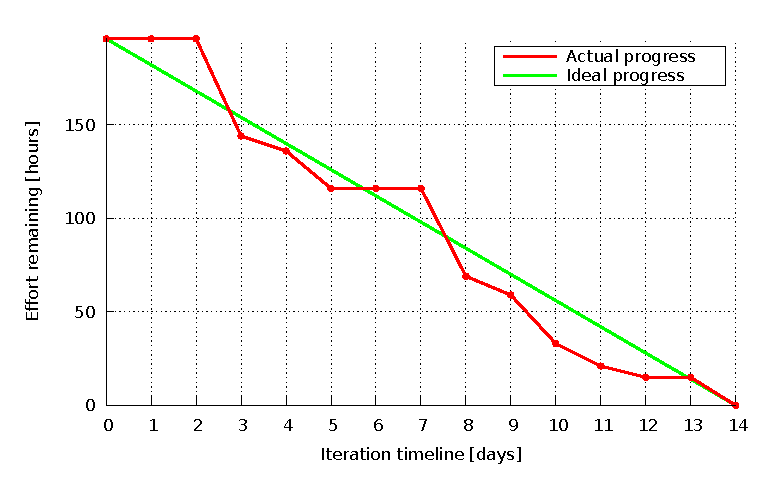
\includegraphics[width=14cm]{burndowns/sprint4.eps}
	\caption{Burn down chart for sprint 4}
	\label{fig:Burn4}
\end{figure}

\subsection{What went well}
All implementation related user stories were finished and as a consequence the goal for sprint 4 and the milestone \emph{Traffic light control} were reached.
The work in implementation part of this project start to escalate and team started to be enthusiastic.

The team was able to prepare and deal with situation, that one member was absent for a whole week.

\subsection{What could be improved}
Stand-up meetings were not that often anymore.
Due to other obligations of all members of team and late attendance during work hours, it was difficult find a common time for these meetings.
Attendance should be more accurate and if absence is known ahead, it should be mentioned to other members.

